\documentclass[12pt]{article}
\usepackage[margin=1in]{geometry}
\usepackage[pdftex]{graphicx}
\usepackage{multirow}
\usepackage{setspace}
\usepackage{enumitem}
\pagestyle{plain}

\begin{document}

% Course information
\noindent
\begin{tabular*}{\textwidth}{l @{\extracolsep{\fill}} r}
  & \multirow{3}{*}{
\includegraphics[height=1.0in]{logo.jpg}} \\
  \large Experimental Techniques & \\
  \large Winter Quarter 2021 & \\
  \large Physics 80 & \\
\end{tabular*}
\vspace{10mm}

% Professor information
\noindent
\begin{tabular}{ l l }
  \multirow{6}{*}{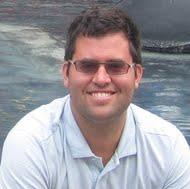
\includegraphics[height=1.25in]{mike.jpg}} & \\
  & \\
  & \large Michael Mulhearn \\
  & \large mulhearn@physics.ucdavis.edu \\
  & \large Physics 317 \\
  & \\
\end{tabular}
\vskip 0.5cm
\noindent
\textbf {Lectures:} M,W 11:00-11:50 AM  Remote Instruction
\begin{tabbing}
\hspace*{3em}\= \hspace*{5em} \= \kill % set the tabbings
\textbf {Lab:}    \> Section 1: \> M,W 12:10-2:30 PM Remote Instruction\\
                  \> Section 2: \> T,R 3:10-5:30 PM Remote Instruction\\
\end{tabbing}

\noindent
\textbf {Text:}  Online lecture notes at {\tt https://www.scipy-lectures.org} plus
lecture notes on RLC circuits and Data Analysis on the course website. \\

\noindent
\textbf{Office Hours:} M 11:00-11:50 AM (lecture zoom session) \\

\noindent
\textbf{Lab Instructor:} Junying Huang (jyghuang@ucdavis.edu) \\

\noindent
\textbf {Course Description:}\\
This course has been substantially revised for remote teaching.
Statistical analysis of experimental data, data analysis using
Scientific Python, computational physics, and analysis of electronic
circuits.  If logistics allow, the course will include experimental
study of electronic circuits using take-home lab kits. \\

\noindent
\textbf{Online Solution Services:}\\
You may not use online solution services for any of the problems
assigned for this course, including homework, labs, quizes, or exams,
To do so is a violation of the UC Davis academic code of conduct
(plagarism and/or unauthorized collaboration) I will deploying several
counter measures designed to discourage the use of these services.  If
monitoring these sites with out department account suggests these
measures have been ineffective, we will have a synchronous final exam.\\

\noindent
\textbf{Lectures:}\\
The lectures will be a hybrid between (optional) synchronous and asynchronous content. Short videos which cover the core lecture content will be posted on the course website.  The Wednesday lecture period will be reserved for optional synchronous informal lecture to review the material, answer questions, and solve example problems.  Please prepare for these lectures by watching the videos and reading the corresponding lecture notes.\\

\noindent
\textbf{Homework:}\\
There will be approximately five homework assignments, based on the
lecture material.  {\bf To minimize the effectiveness of cheating, homework
scores will be based solely on whether a legitimate attempt was made.}
Homework and due dates will be posted on the course website.  You may
collaborate on homework problems, but each student should provide
their own solution.\\

\noindent
\textbf{Midterm Exams:} There will be one or more take-home midterm exams. \\

\noindent
\textbf{Final Exam:}\\
The final exam will be take-home, unless I find
evidence that the take-home exams have been compromised.  For this reason, reserve the scheduled final exam slot:  Mar 17, 2021 at 10:30 AM.\\

\noindent
\textbf {Lab Activities:}\\
The lab activities are the most important component of this course.
The lab activities have been redesigned to accommodate remote
instruction.  They may be completed asynchronously, but the lab TA
will be available remotely during your scheduled lab section to
answer questions.  You may work alone or in groups of two.  Groups of
three will be allowed, with lab TA permission, in exceptional
circumstances.\\

\noindent
\textbf {Logbooks:}\\ 
Most scientist these days employ a mixture of handwritten and digital
logbooks.  Quick notes and sketches about procedures, calculations,
and the results of simple measurements are often most conveniently
handwritten.  Extensive data collection and detailed analysis are
usually done entirely on a computer.  You should keep a hand-written
log book for the quick notes, but in some cases, you will be asked to
keep an ASCII text file as a simple digital logbook.\\

\noindent
\textbf {Jupyter Notebooks:}\\
Most of the lab assignments involve the completion of a Jupyter
Notebook.  Each lab partner should write their own notebook, but you
may share your working code.  Place the name of the lab, the date of
the lab, and the name of your lab partners in the first cell as a
comment, even though you are each keeping your own notebook.

Start each of your notebooks with the magic python function
{\tt\%pylab inline} to load numpy as np, matplotlib as plt, and show
plots as cell output (inline).

Make sure all of your output is visible, print your notebook as a PDF
file, and post the PDF file to the course web site. Each Jupyter
Notebook will be graded on a 100 point scale.\\

\newpage

\noindent
\textbf {Course Schedule}:\\
Note that the dates refer to lectures.  For section 2, the lab date is
the next day, so e.g. the ``Plotting'' lab is on 14 Jan.  The topics
and schedule may be adjusted while the course is in progress.  The
lecture refer to chapters in the lecture notes for Analysis (A), Fourier (F), and Passive Electronics (P), so, e.g. ``A1'' is ``Analysis of Experimental Data, Chapter 1''.

\begin{table}[h!]
\normalsize % The size of the table text can be changed depending on content. Remove if desired.
\begin{tabular}{ lllll }
\hline
\textbf{Week} & \textbf{Date} & \textbf{Lecture} & \textbf{Lab} \\
\hline
1 & 4 Jan & (async)       & (no lab) \\
  & 6 Jan & (async)       & (no lab)\\
\hline
2 & 11 Jan & (async)      & Intro. to Scipy \\
  & 13 Jan & Recap A. 1   & Plotting \\
\hline
3 & 20 Jan & (async)      & (catch-up) \\
\hline
4 & 25 Jan & (async)      & The Monte Carlo method\\
  & 27 Jan &              & (catch-up)\\
\hline
5 & 1 Feb  & (async)      & Limits of Distributions\\
  & 3 Feb  & Recap A. 2   & (catch-up)\\
\hline
6 & 8 Feb  & (async)      & Uncertainties\\
  & 10 Feb & Problems     & (catch-up)\\
\hline
7 & 17 Feb  & Recap A.3   & (catch-up)\\
\hline
8 & 22 Feb  & (async)     & Curve Fitting \\
  & 24 Feb  & Pre-cap P.1 & Ideal Gas\\
\hline
9 & 1 Mar   & (async)     & (catch-up) \\
  & 3 Mar   & Pre-cap P.2 & (catch-up) \\
\hline
10 & 8 Mar  & (async)     & TBD \\
   & 10 Mar & Review      & (catch-up) \\
\hline
\end{tabular} 
\end{table}

\end{document}

